\section{General-purpose Counterfactuals}
\label{sec:general_purpose}



\newcommand{\tagdefine}[1]{\emph{{\color{darkgray}#1} }}
%\renewcommand{\arraystretch}{1.1}
\newcommand{\TagTable}{
\begin{table*}
\small
\centering
\begin{tabular}{@{} p{0.11\linewidth} p{0.61\linewidth}  p{0.22\linewidth} @{}}
\toprule
\textbf{\Tagstr} & \textbf{Definitions and \sysname-generated Examples} & \textbf{Training Datasets} \\ 
\midrule
\ctrltag{negation}
    & A dog is \add{not} embraced by the woman.
    & \cite{kaushik2019learning}
\\ \midrule
\ctrltag{quantifier}
    & \swap{A dog is}{Three dogs are} embraced by the woman. 
    & \cite{gardner2020contrast}
\\ \midrule
\ctrltag{shuffle}
    & \tagdefine{To move (or swap) key phrases or entities around the sentence.} \newline
    A \swap{dog}{woman} is embraced by the \swap{woman}{dog}.
    & \cite{zhang2019paws}
\\ \midrule
\ctrltag{lexical}
    & \tagdefine{To change just one word or noun chunks without breaking the POS tags.} \newline
      A dog is \swap{embraced}{attacked} by the woman.
    & \cite{sakaguchi2019winogrande}
\\ \midrule
\ctrltag{resemantic}
    & \tagdefine{To replace short phrases or clauses without affecting the parsing tree.}\newline
      A dog is \swap{embraced by the woman}{wrapped in a blanket}.
    & \cite{wieting2017paranmt}
\\ \midrule
\ctrltag{insert}
    & \tagdefine{To add constraints without affecting the parsing structure of other parts.} \newline
      A dog is embraced by the \add{little} woman.
    & \cite{mccoy2019right}
\\ \midrule
\ctrltag{delete}
    & \tagdefine{To remove constraints without affecting the parsing structure of other parts.} \newline
    A dog is embraced \remove{by the woman}.
    & \cite{mccoy2019right}
\\ \midrule
\ctrltag{restructure}
    & \tagdefine{To alter the dependency tree structure, \eg changing from passive to positive.} \newline
    A dog is \swap{embraced by}{hugging} the woman.
    & \cite{wieting2017paranmt}
\\
\bottomrule
\end{tabular}
\vspace{-5pt}
\caption{A list of \tagstrs used for semantically driving the counterfactual generation in \sysname, their examples, and the representative training datasets for the corresponding patterns. %More examples are in Appendix~\ref{appendix:example}.
}
%\wts{Change all the examples to be on an identical sentence, not all different cases. And consider further annotate the tags based on whether they just do semantic change or also syntactic change.}}
\label{table:ctrltag}
\vspace{-10pt}
\end{table*}
}
% on a particular instance
% 
\subsection{Definition and Desiderata}
\label{sec:desiderata}


Given an instance $x \in \xset$, a generator $g$ produces a set of counterfactuals $\hat{\xset} = \{\xp_1, \xp_2, ...\}$ with various relationships $x \veryshortarrow \xp_i$ (referred as $\relation{\xp_i}$ for simplicity).
% Each $\xp_i$ perturbs $x$ with certain strategies like negations, syntactic restructuring, etc., and the edited spans are instantiations of the strategies.
For example, \swap{great}{not great}, \swap{kids}{no one} in Figure~\ref{fig:teaser}B are both instances of the \ctrltag{negation} relationship.
% The importance of certain $\relation{\xp}$ changes along with applications.
Relationships are not mutually exclusive -- these counterfactuals are also instances of the \emph{label flipping} relationship if the task is sentiment analysis (but might not be for other tasks).
As illustrated in \S\ref{sec:intro}, knowledge of such relationships aids selections for downstream applications.
% this sentence is totally unecessary
% We now turn to desiderata for general-purpose counterfactuals: closeness, fluency, diversity, and controllability.
% \emph{Independent of the application}, we prefer $\xp$ with the following four desiderata: closeness, fluency, diversity, and controllability.
%which inspire our modeling in \S\ref{subsec:nlg}:
% Knowledge of such relationships aid downstream filtering and ranking.
% $\relation{\xp}$ then forms certain relationships that are useful for downstream filtering (\eg perturbation strategy, the added and removed tokens, the impacts on groundtruth label, model prediction, etc.)
%The perturbation follow certain \emph{strategies} $s$ (e.g., negations~\cite{kaushik2019learning}, word substitution~\cite{li-etal-2020-bert-attack}, syntactical restructing~\cite{iyyer2018adversarial}).

We expect $g$ to produce counterfactuals $\xp$ that are (1) \textbf{close} to $x$, preferably only involving the minimal changes necessary to establish a certain effect~\cite{pearl2018causal}, to allow causality assessments about $\relation{\xp}$.
The generated $\xp$ should also be (2) \textbf{fluent}, \ie grammatically correct~\cite{morris2020textattack} and semantically meaningful (\eg \exinline{Colorless green ideas sleep furiously} is not meaningful~\cite{chomsky2002syntactic}).
Fluency operationalize ``probable'' counterfactuals in the context of NLP;
As \citet{kahneman} stated, humans strongly favor counterfactuals that are close to the original instance, but also prefer those that could have easily happened without assuming rare events or strange coincidences.
%Humans strongly favor counterfactuals that are close to the original instance, but also prefer them to be probable, \ie they could have easily happened without assuming rare events or strange coincidences~\cite{kahneman}.
%We operationalize ``probable'' in the context of NLP by requiring $g$ to generate (2) \textbf{fluent} $\xp$, \ie grammatically correct~\cite{morris2020textattack} and semantically meaningful (\eg \exinline{Colorless green ideas sleep furiously} is not meaningful~\cite{chomsky2002syntactic}).
Further, as a general-purpose generator, $g$ should generate counterfactuals with a measure of (3) \textbf{control} over relationships $\relation{\xp}$, such that counterfactuals vary with the object of attention depending on the application at hand (the ``focus rule''~\cite{kahneman}).
Finally, %even though infinite diverse counterfactuals can be produced \cite{pearl2018causal},
we expect $g$ to output a (4) \textbf{diverse} set of $\xp$ in terms of relationships, so as to cover the large variety of ``what-ifs'' in different applications~\cite{pearl2018causal}.


%A counterfactual $\xp$ should be \textbf{close} to $x$, preferably only involving the minimal changes necessary to establish a certain effect~\cite{pearl2018causal}  for causality assessments about $\relation{\xp}$. 
%Humans strongly favor counterfactuals that are close to the original instance~\cite{kahneman}, while also being probable, \ie which could have easily happened without assuming rare events or strange coincidences.
%We operationalize ``probable'' in the context of NLP by requiring $\xp$ that are \textbf{fluent}, \ie grammatically correct~\cite{morris2020textattack} and semantically meaningful (\eg \exinline{Colorless green ideas sleep furiously} is not meaningful~\cite{chomsky2002syntactic}).
%A general-purpose generator should be able to generate counterfactuals with a measure of \textbf{control} over relationships $\relation{\xp}$, such that counterfactuals vary with the object of attention depending on the application at hand (the ``focus rule''~\cite{kahneman}).
%Finally, we expect the output set $\hat{\xset}$ to be \textbf{diverse} in terms of relationships, so as to support diverse applications.

% Meanwhile, we also expect to collect sets with (4) \textbf{controlled} $\relation{\xp}$ relationships.
% The control is essential to support a wide range of specific applications, \eg counterfactual explanations on salient features (\S\ref{sec:app_explain}), error analyses that group semantically or syntactically related $\xp$ (\S\ref{sec:app_err_analysis}), etc.
% It reflects the ``focus rule''~\cite{kahneman}: counterfactuals would vary with the object of attention.
%, even when the same variable is acted upon.
%Following common practice in NLP research, we estimate \emph{closeness} using the semantic and syntactic distance between $x$ and $\xp$~\cite{morris2020textattack, madaan2020generate}.
% However, $\xp$ also needs to be (2) \textbf{fluent}, \ie grammatically correct~\cite{morris2020textattack} and semantically meaningful (\eg \exinline{It's scary for water} is not meaningful.)
% This estimates the likelihood of a sentence occurring in reality; as \citet{kahneman} stated, the counterfactual scenario should be one that could have easily happened without rare assumptions. 
%In NLP, this translates to sentences that are likely to be written.


%However, $\xp$ also needs to be realistic, \ie the counterfactual scenario should be one that could have easily happened, without rare assumptions or coincidences~\cite{kahneman}. 
%In NLP, this translates to sentences that are likely to be written, \ie (2) \emph{fluent} counterfactuals that are grammatically correct~\cite{morris2020textattack} and semantically meaningful (\eg \exinline{It's scary for water} is grammatically correct but not meaningful.) 

% Since there can be an infinite number of ``what-ifs'' \cite{pearl2018causal}, we also consider properties of $\hat{\xset}$, the produced \emph{set of counterfactuals}.

% Since our goal is to produce a general-purpose set of counterfactuals, we expect the set to be (3) \textbf{diverse} in terms of relationships between $x$ and $\xp$.
%However, when the targeted relationship is unclear, an approximation could be the similarity of counterfactuals \emph{to each other} (using \eg self-BLEU~\cite{Hu2017TowardCG}).
%, and also to contain various instantiations of the same relationship.
% Meanwhile, we also expect to collect sets with (4) \textbf{controlled} $\relation{\xp}$ relationships.
% The control is essential to support a wide range of specific applications, \eg counterfactual explanations on salient features (\S\ref{sec:app_explain}), error analyses that group semantically or syntactically related $\xp$ (\S\ref{sec:app_err_analysis}), etc.
% It reflects the ``focus rule''~\cite{kahneman}: counterfactuals would vary with the object of attention.
%Additionally, augmentations usually prioritize (3) \emph{diversity} --- a group of $x$s are preturbed using various strategies, and various initiations under the same strategy, such that they provide different constraints on finetuning decision boundaries.
%On the other hand, evaluations and explanations require more (4) \emph{controlled} perturbations for systematic and targeted inspections.
%The diversity and the controllability are two competing factors, and prior work focusing on certain applications follow one of two extremes.
%Those that thrive in diversity are either too uncontrolled (\eg text generation~\cite{iyyer2018adversarial}) or hard to scale (\eg manual rewrites~\cite{kaushik2019learning, gardner2020contrast}), whereas those that rely on templates or heuristic rules usually only cover limited linguistic patterns~\cite{li2020linguistically}.


\begin{figure}[t]
\centering
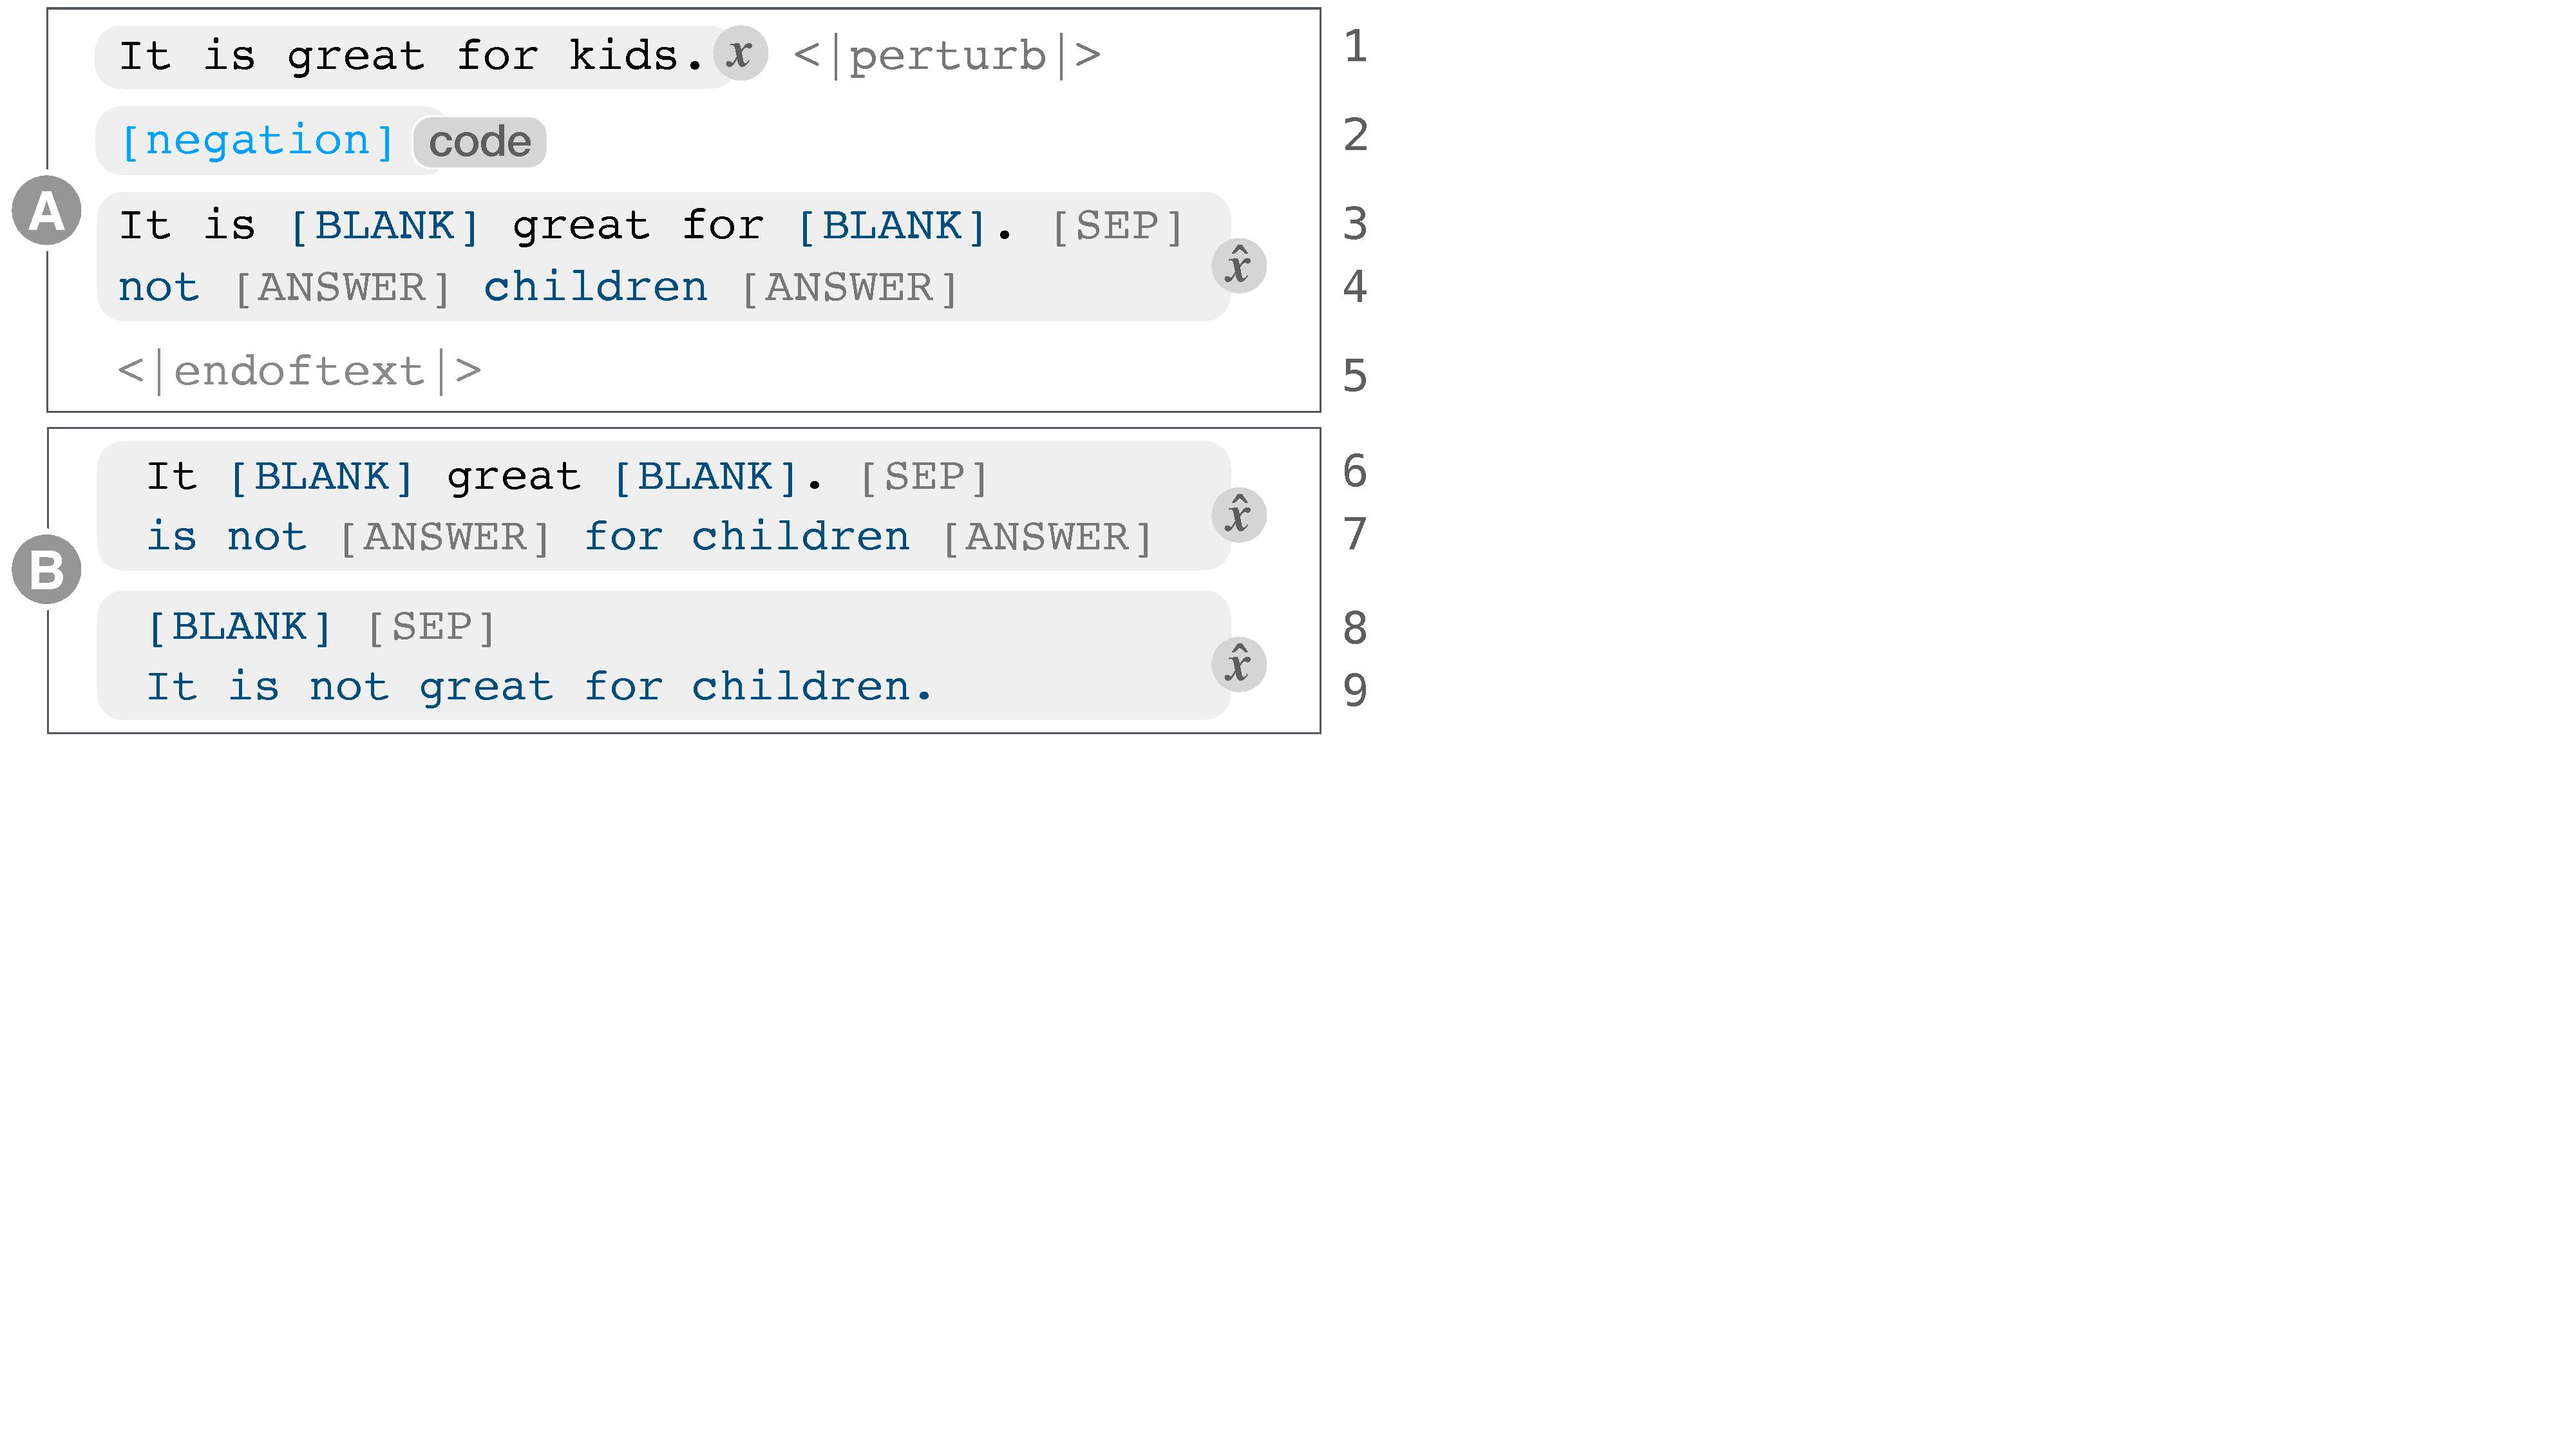
\includegraphics[trim={0 18.6cm 31.5cm 0cm}, clip, width=1\columnwidth]{figures/blank.pdf}
\vspace{-15pt}
\caption{  
(A) The text format for \sysname, which concatenates the original $x$, the \tagstr, and the $\xp$ (converted to the infilling structure from \exinline{It is not great for children}).
At \emph{generation} time, \sysname accepts prompts that just include $x$ (Line 1), or with the \tagstrshort and the \texttt{BLANK}s (Line 2--3).
During training, the \tagstrshorts and blanks are automatically extracted.
(B) The blanking structure can flexibly cover just the $\xp$ subtrees that contain the change, or the entire sentence, such that Line 3--4 in (A) can be replaced by Line 6--7 or 8--9.
%We get multiple training texts per pair, by blanking $\xp$ subtrees that contain the change, or the entire sentence.
}
\vspace{-10pt}
\label{fig:blank}
\end{figure}


\subsection{Modeling through Text Generation}
\label{subsec:nlg}


\TagTable

\paragraph{\emph{Closeness} and \emph{Controllability}: Conditional text generation.}
%1. We frame it as conditional text generation. We always condition on the original x (line 1)
%2. Control codes: explain what they are , reference table 1, etc (line 2)
%3. Blanking: we extend ILM, etc. This is why it's nice, etc (line 3).
%4. Control codes & blanking allow for control, but they are optional: the generator can generate them based on the original x

We frame counterfactual generation as a conditional text generation task using language models (LMs), and wrap the \emph{conditions} into textual prompts as in Figure~\ref{fig:blank}.
First, to ensure $g$ generates $\xp$ that are \emph{close} to $x$ (rather than arbitrary text), we build mappings between paired, and always condition the generation on the original $x$ (Line 1).

Second, to achieve the control on $\relation{\xp}$, we include \emph{\tagstrs} (\eg \ctrltag{negation} in Line 2), which encode the type of perturbations.
Inspired by prior work categorizing manually created counterfactuals~\cite{kaushik2019learning, gardner2020contrast}, we design eight \tagstrshorts (Table~\ref{table:ctrltag}) that distinguish lexical, syntactic, and semantic perturbations.

Besides the perturbation types, we additionally control where changes happen.
We extend the Infilling by Language Modeling (ILM) framework~\cite{donahue2020enabling}, such that $\xp$ contains \texttt{[BLANK]} tokens where perturbations are to be applied (Line 3). 
As shown in Figure~\ref{fig:blank}B, Lines 6--9, ILM allows for perturbations of any length (additions and deletions) beyond single word substitutions.

At generation time, with Line 2 and 3 specified, \sysname can just fills in the blanks sequentially according to the controls (Line 4).
However, the control conditions are optional.
When we exclusively condition the generation on $x$ (Line 1), \sysname can generate Line 2--3 on its own by sampling the \tagstr and the location of blanks.



\paragraph{\emph{Diversity}: Combining multiple paired sentences.}
Large pre-trained LMs like GPT-2~\cite{radford2019language} naturally increase the semantic and syntactic \emph{diversity} over word substitutions~\cite{garg2019counterfactual} and templates~\cite{ribeiro2018sear}.
We further finetune GPT-2 on six existing datasets of paired sentences, each containing counterfactuals with a subset of the \tagstrs of interest (see Table~\ref{table:ctrltag}). 
Additionally, we find naturally occurring pairs in non-paired datasets like SQAuD~\cite{rajpurkar-etal-2016-squad}, using heuristics on the editing distance. 
%We use the pairs as negative samples if the change is too extensive.
A combination of these datasets yields a model that can produce \emph{diverse} counterfactuals.

We translate each paired $(x, \xp)$ into the prompt format in Figure~\ref{fig:blank}. 
We compute the primary \tagstrshort based on linguistic features such as part-of-speech tags or dependency trees, and verify through an ablation study in Appendix~\ref{appendix:ablation_control} that training \sysname with \tagstrs greatly improves the success rate when generating counterfactuals that have these properties by 8\%--64\%.
To allow flexible blanking, we also vary the location of \texttt{[BLANK]}s according to the example's parse tree.
As a result, form $657,144$ training prompts from $191,415$ sentence pairs. 
More training prompt details and \tagstrshort statistics are in Appendix~\ref{appendix:train_data}.

Similar to \citet{madaan2020generate}, we quantitatively compare \sysname generations with baseline models.
As Appendix~\ref{appendix:intrinsic} summarizes, \sysname generates $\xp$ that are closer to $x$ than a standard generative model~\cite{Dathathri2020Plug} (\ie with much smaller syntactic editing distance~\cite{zhang1989simple}), and more diverse than off-the-shelf masked models like RoBERTa~\cite{liu2019roberta} (quantified using self-BLEU~\cite{zhu2018texygen}).


\paragraph{\emph{Fluency}: Through post-hoc filtering.}
Certain combinations of \tagstrs and \texttt{BLANK}s cause \sysname to generate ungrammatical or nonsensical counterfactuals 40\% of the time.
Similar to \citep{morris2020textattack}, we score both $x$ and $\xp$ using non-finetuned GPT-2, and filter out $\xp$ if its log-probability (either on the full sentence or on the perturbed chunks) decreases more than 10 points relative to $x$.
Because our applications in \S\ref{sec:app_label}--\S\ref{sec:app_err_analysis} all involve human teammates double checking the generation from \sysname, we intentionally select this loose threshold to present more \emph{diverse} counterfactuals. 
As further illustrated in \S\ref{subsec:label_efficiency}, we verify through human evaluation that the filtering improves the portion of fluent generations to 70\%--80\%, which we deem reasonable for the human to further inspect.
If used in a purely automated setting (\eg adversarial attack), we can use stricter constraints~\cite{morris2020textattack} to improve fluency, at the cost of diversity --- rarer and more surprising changes may be blocked even if they are fluent. 








